\appendix

\section{Appendix}

Runtime may be affected by other processes running on the machine, since it was my personal computer. They are listed here for reference.

\subsection{Baseline runs}

\begin{table}[H]
\caption{Network architecture sweep results (baseline)}
\label{appendix:baseline}
\centering
\begin{adjustbox}{center}

\begin{tabular}{@{} cccccccccc @{}} \toprule
\multirow{2}{*}{\bf Feature set} &
\multicolumn{3}{c}{\bf Train hyperparams} &
\multicolumn{2}{c@{}}{\bf Network} &
\multirow{2}{*}{\makecell{\bf Val loss\\\textit{min}}} &\multirow{2}{*}{\makecell{\bf Rating\\\textit{elo (avg=0)}}} &\multirow{2}{*}{\makecell{\bf Puzzles\\\textit{move acc.}}} &
\multirow{2}{*}{\makecell{\bf Runtime\\\textit{hh:mm:ss}}} \\
\cmidrule(lr){2-4} \cmidrule(l){5-6}
& \bf Batch & \bf LR & \bf Gamma & \bf L1 & \bf L2 & \\
\midrule
    \featureset{HV} & 16384 & 5e-04 & 0.99 & 256 & 32 & 0.00351 & 89.8 $\pm$ 7.3 & \textbf{0.9047} & 1:53:59 \\
\featureset{HV} & 16384 & 5e-04 & 0.99 & 256 & 64 & 0.00342 & 16.5 $\pm$ 7.4 & 0.8976 & 1:54:56 \\
\featureset{HV} & 16384 & 5e-04 & 0.99 & 256 & 128 & 0.00330 & -42.8 $\pm$ 7.6 & 0.8885 & 1:52:29 \\
\featureset{HV} & 16384 & 5e-04 & 0.99 & 256 & 256 & 0.00319 & -65.5 $\pm$ 7.5 & 0.8826 & 2:29:26 \\
\featureset{HV} & 16384 & 5e-04 & 0.99 & 512 & 32 & 0.00309 & 106.6 $\pm$ 7.4 & 0.9027 & 1:54:28 \\
\featureset{HV} & 16384 & 5e-04 & 0.99 & 512 & 64 & 0.00300 & 50.7 $\pm$ 8.2 & 0.8975 & 1:53:44 \\
\featureset{HV} & 16384 & 5e-04 & 0.99 & 512 & 128 & 0.00290 & 12.4 $\pm$ 7.0 & 0.8880 & 1:51:06 \\
\featureset{HV} & 16384 & 5e-04 & 0.99 & 512 & 256 & 0.00279 & -68.9 $\pm$ 8.6 & 0.8790 & 1:51:17 \\
\featureset{HV} & 16384 & 5e-04 & 0.99 & 1024 & 32 & 0.00268 & \textbf{115.1 $\pm$ 8.6} & 0.9032 & 2:15:18 \\
\featureset{HV} & 16384 & 5e-04 & 0.99 & 1024 & 64 & 0.00265 & 52.5 $\pm$ 7.7 & 0.8955 & 2:03:41 \\
\featureset{HV} & 16384 & 5e-04 & 0.99 & 1024 & 128 & 0.00257 & -19.5 $\pm$ 8.6 & 0.8852 & 2:06:39 \\
\featureset{HV} & 16384 & 5e-04 & 0.99 & 1024 & 256 & 0.00246 & -112.1 $\pm$ 8.6 & 0.8725 & 2:32:47 \\
\featureset{HV} & 16384 & 5e-04 & 0.99 & 2048 & 32 & 0.00241 & 102.1 $\pm$ 9.1 & 0.8968 & 3:11:56 \\
\featureset{HV} & 16384 & 5e-04 & 0.99 & 2048 & 64 & 0.00238 & 29.3 $\pm$ 7.2 & 0.8876 & 3:12:46 \\
\featureset{HV} & 16384 & 5e-04 & 0.99 & 2048 & 128 & 0.00234 & -77.5 $\pm$ 7.1 & 0.8779 & 3:29:07 \\
\featureset{HV} & 16384 & 5e-04 & 0.99 & 2048 & 256 & \textbf{0.00221} & -188.8 $\pm$ 8.2 & 0.8678 & 3:27:47 \\
\bottomrule \end{tabular}

\end{adjustbox}
\end{table}

\begin{figure}[H]
\centering
\makebox[\textwidth]{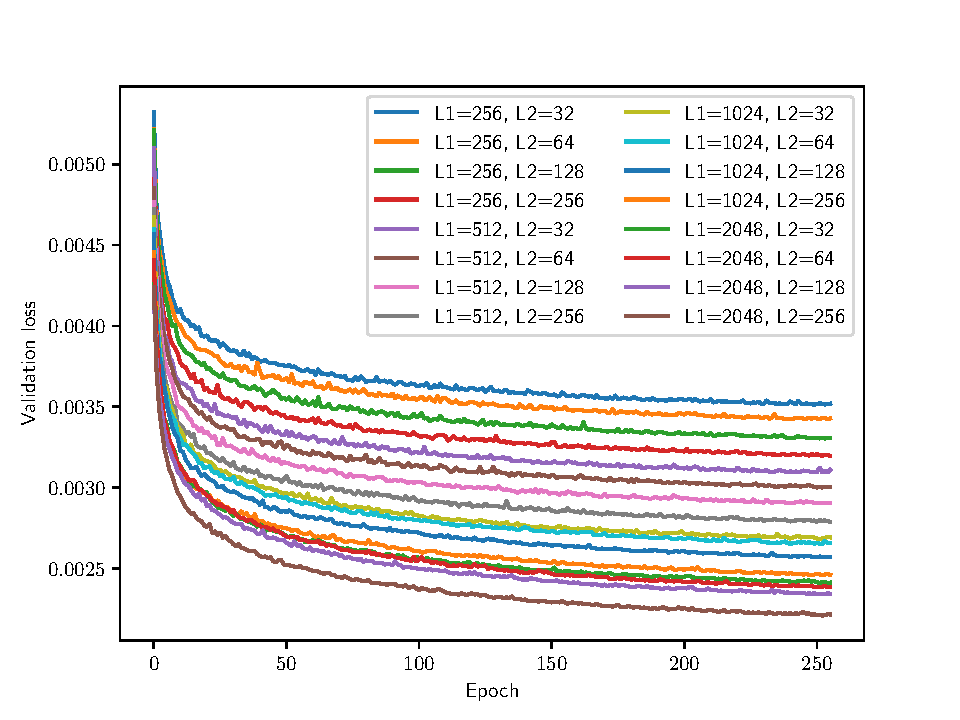
\includegraphics[width=\textwidth]{./dynamic/output/baseline_val_loss.pdf}}
\caption{Network architecture sweep validation loss over epochs (baseline)}
\end{figure}

\newpage
\subsection{Axis encoding examples}
\label{appendix:axis_samples}

\begin{figure}[h]
\centering
\subfloat[\centering $\white$ White]{{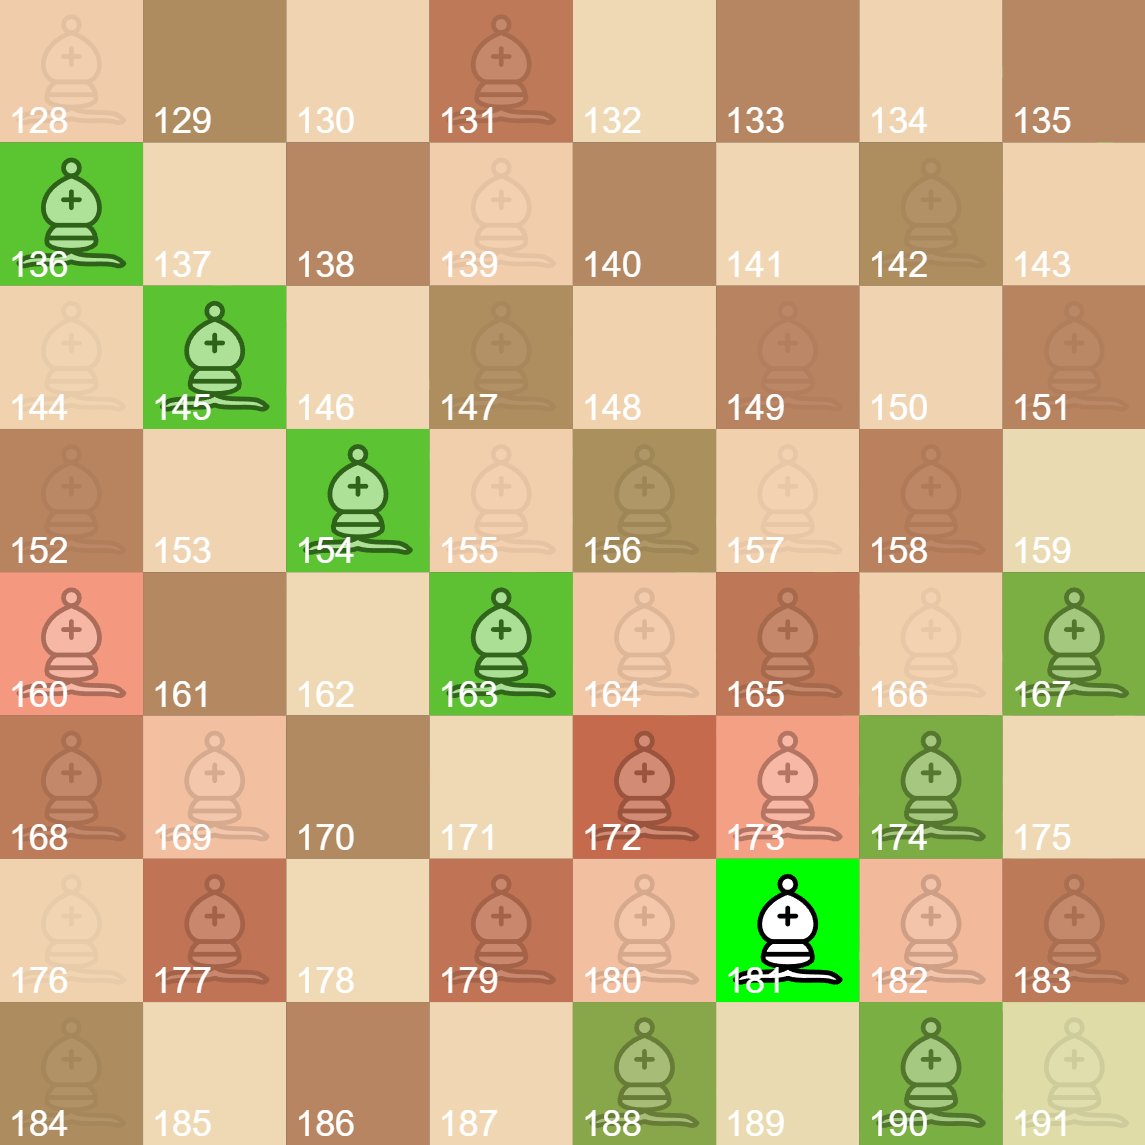
\includegraphics[width=4.65cm]{../assets/results/piece_weights/white_bishop_weights.png} }}
\qquad
\subfloat[\centering $\white$ White]{{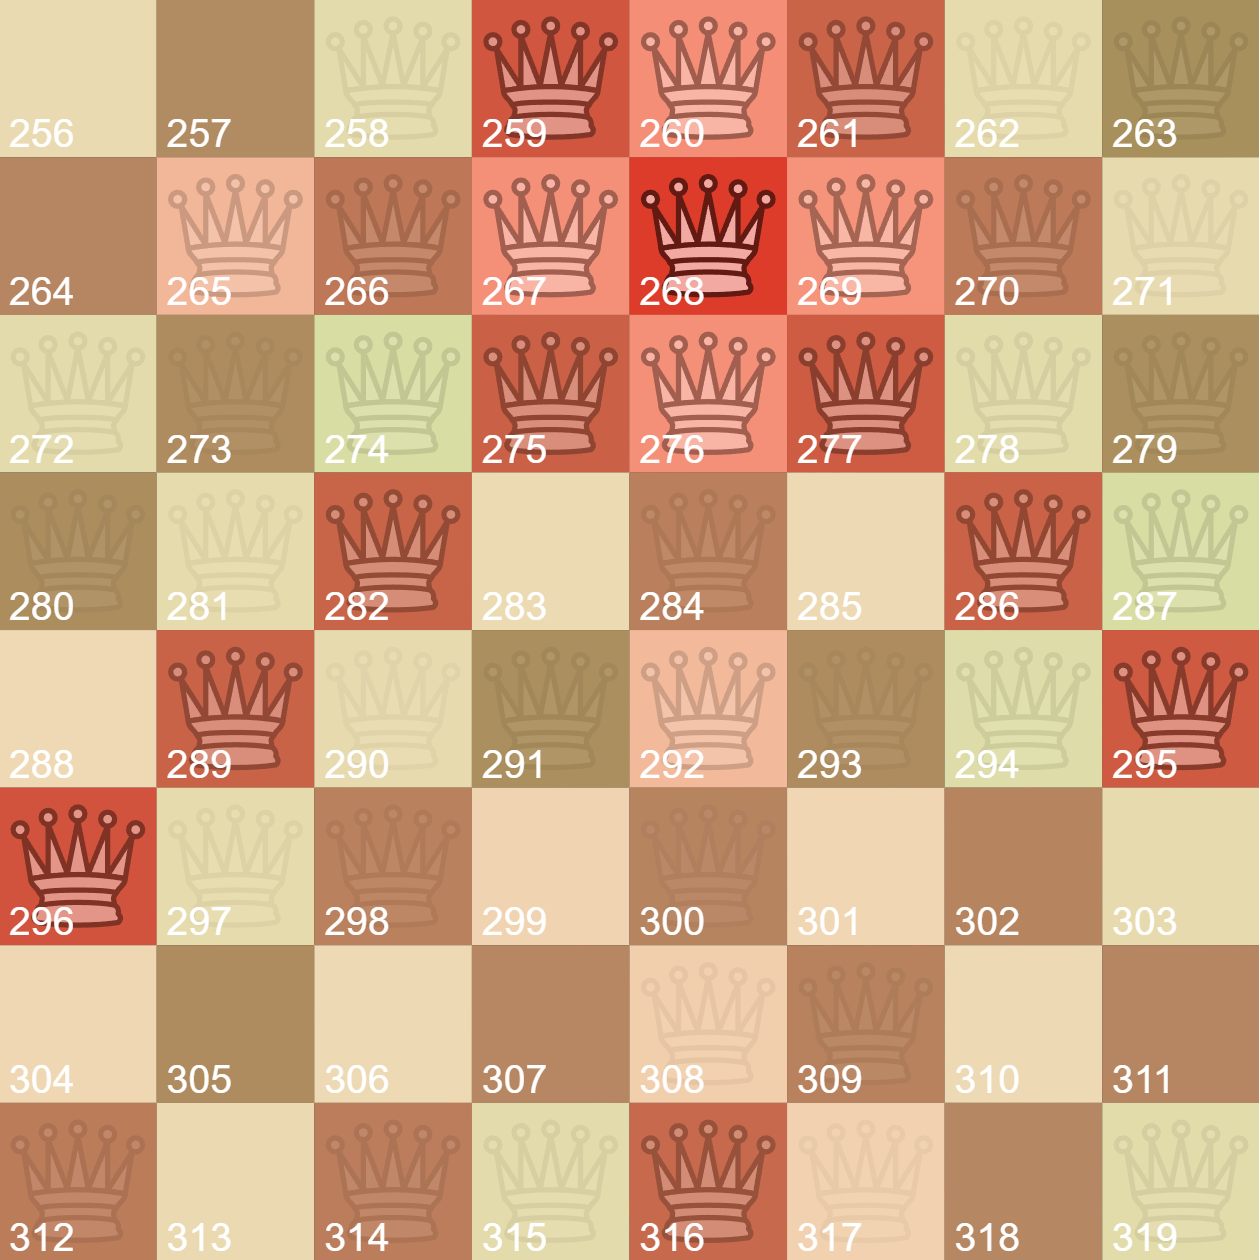
\includegraphics[width=4.65cm]{../assets/results/piece_weights/white_queen_weights.png} }}
\qquad
\subfloat[\centering $\white$ White]{{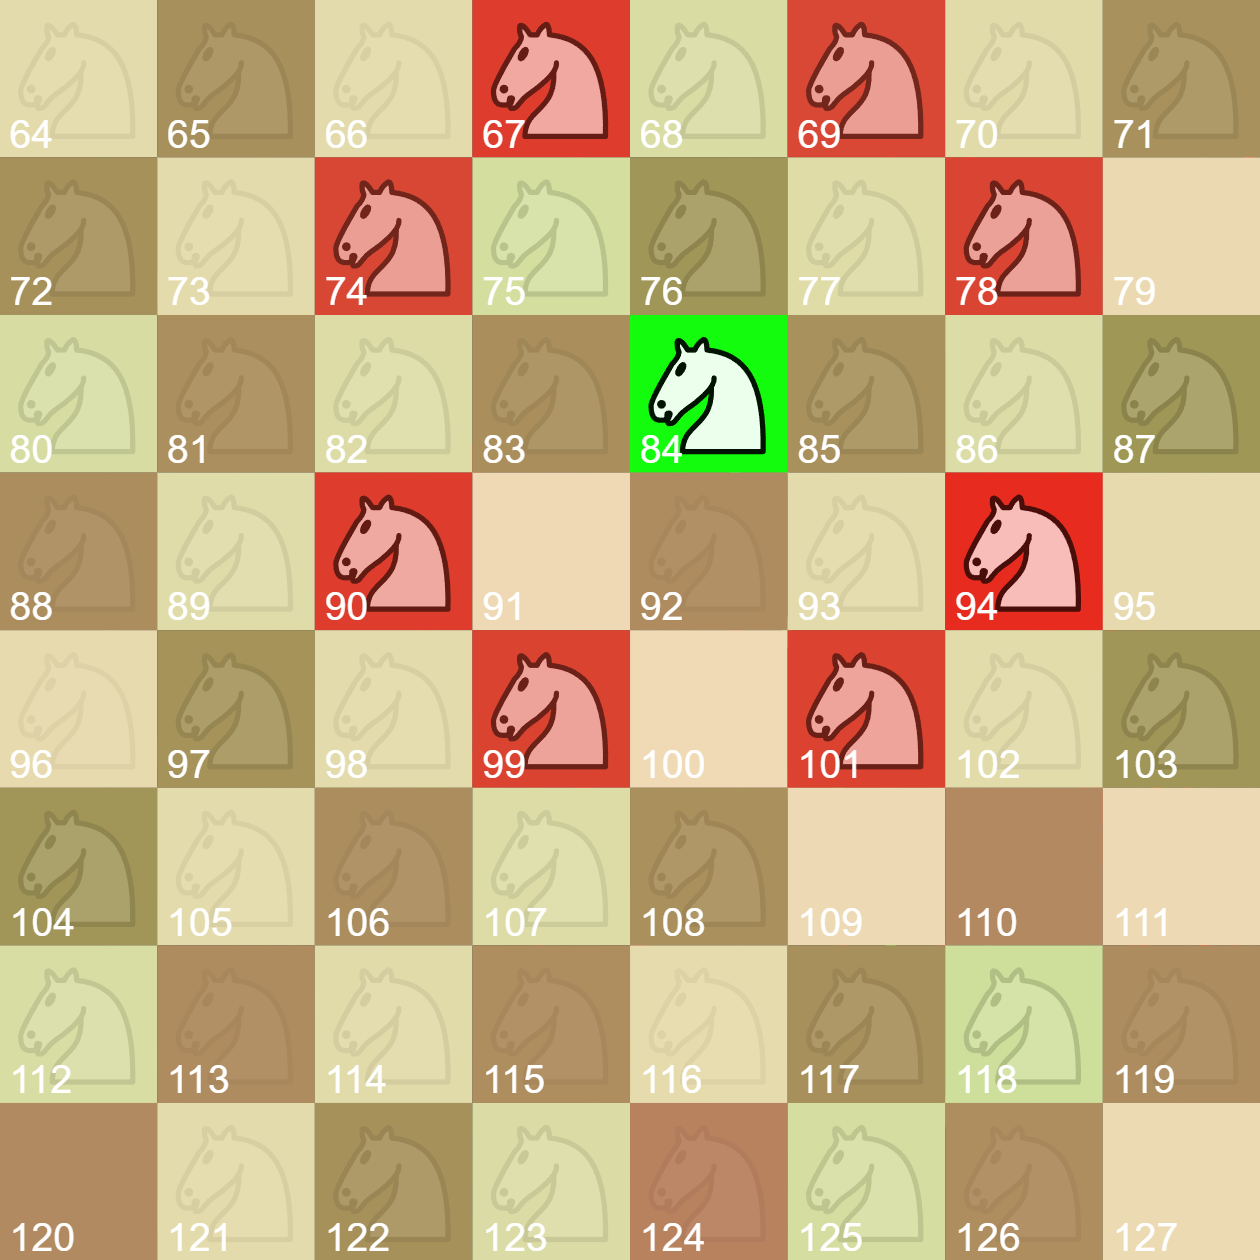
\includegraphics[width=4.65cm]{../assets/results/piece_weights/white_knight_weights.png} }} \\

\subfloat[\centering $\black$ Black]{{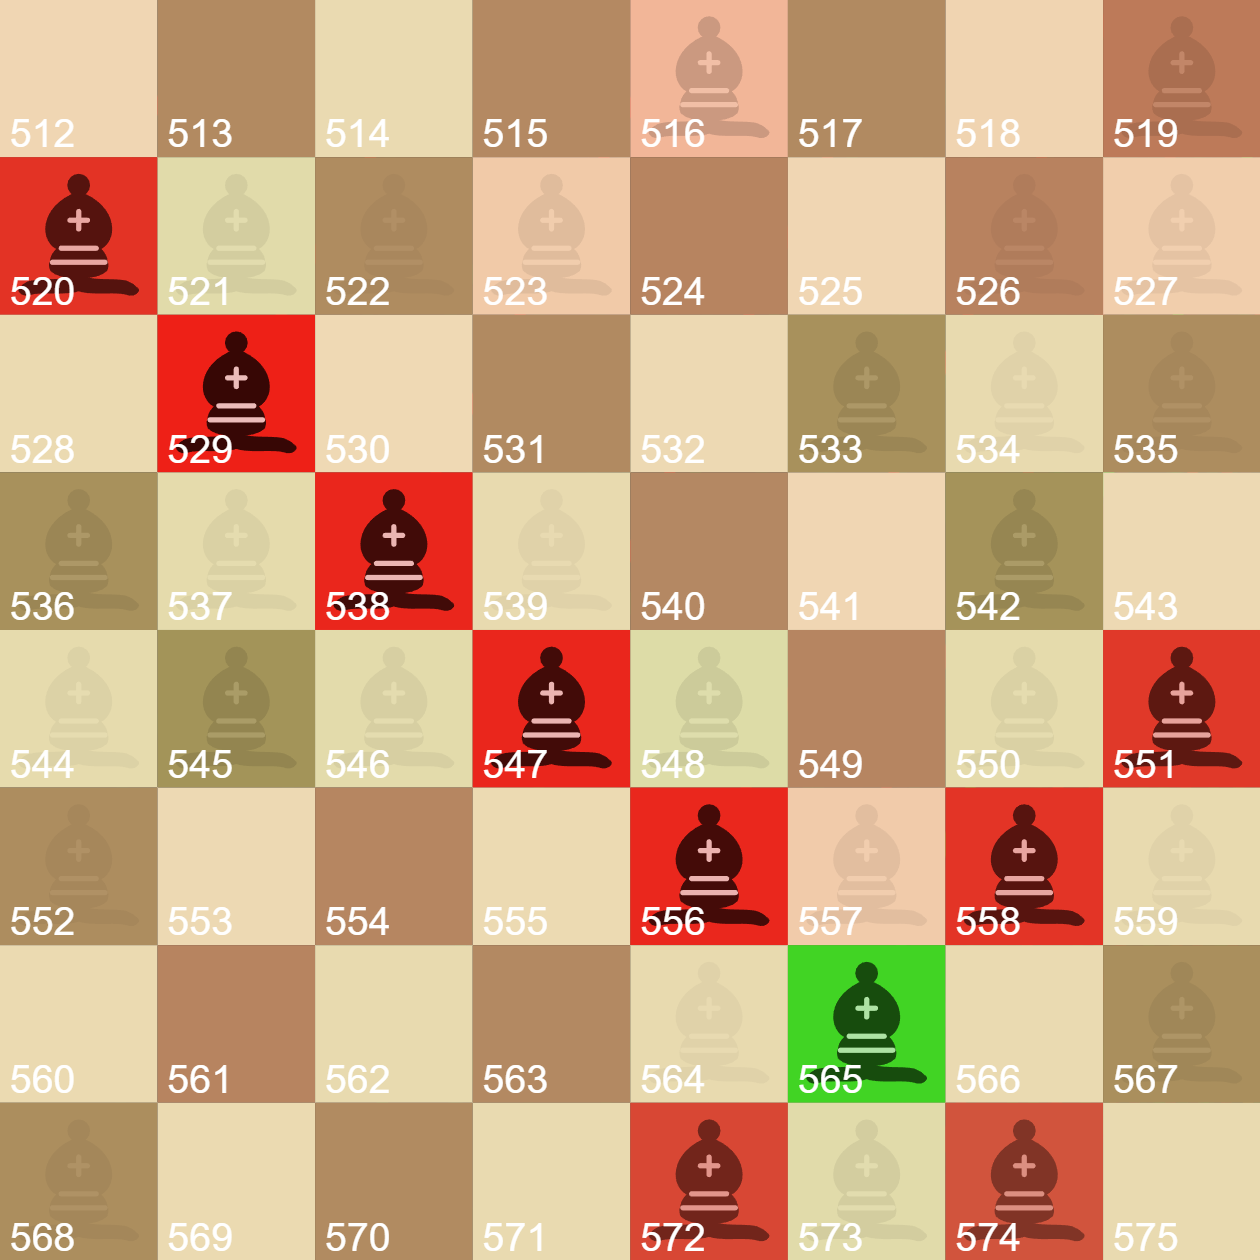
\includegraphics[width=4.65cm]{../assets/results/piece_weights/black_bishop_weights.png} }}
\qquad
\subfloat[\centering $\black$ Black]{{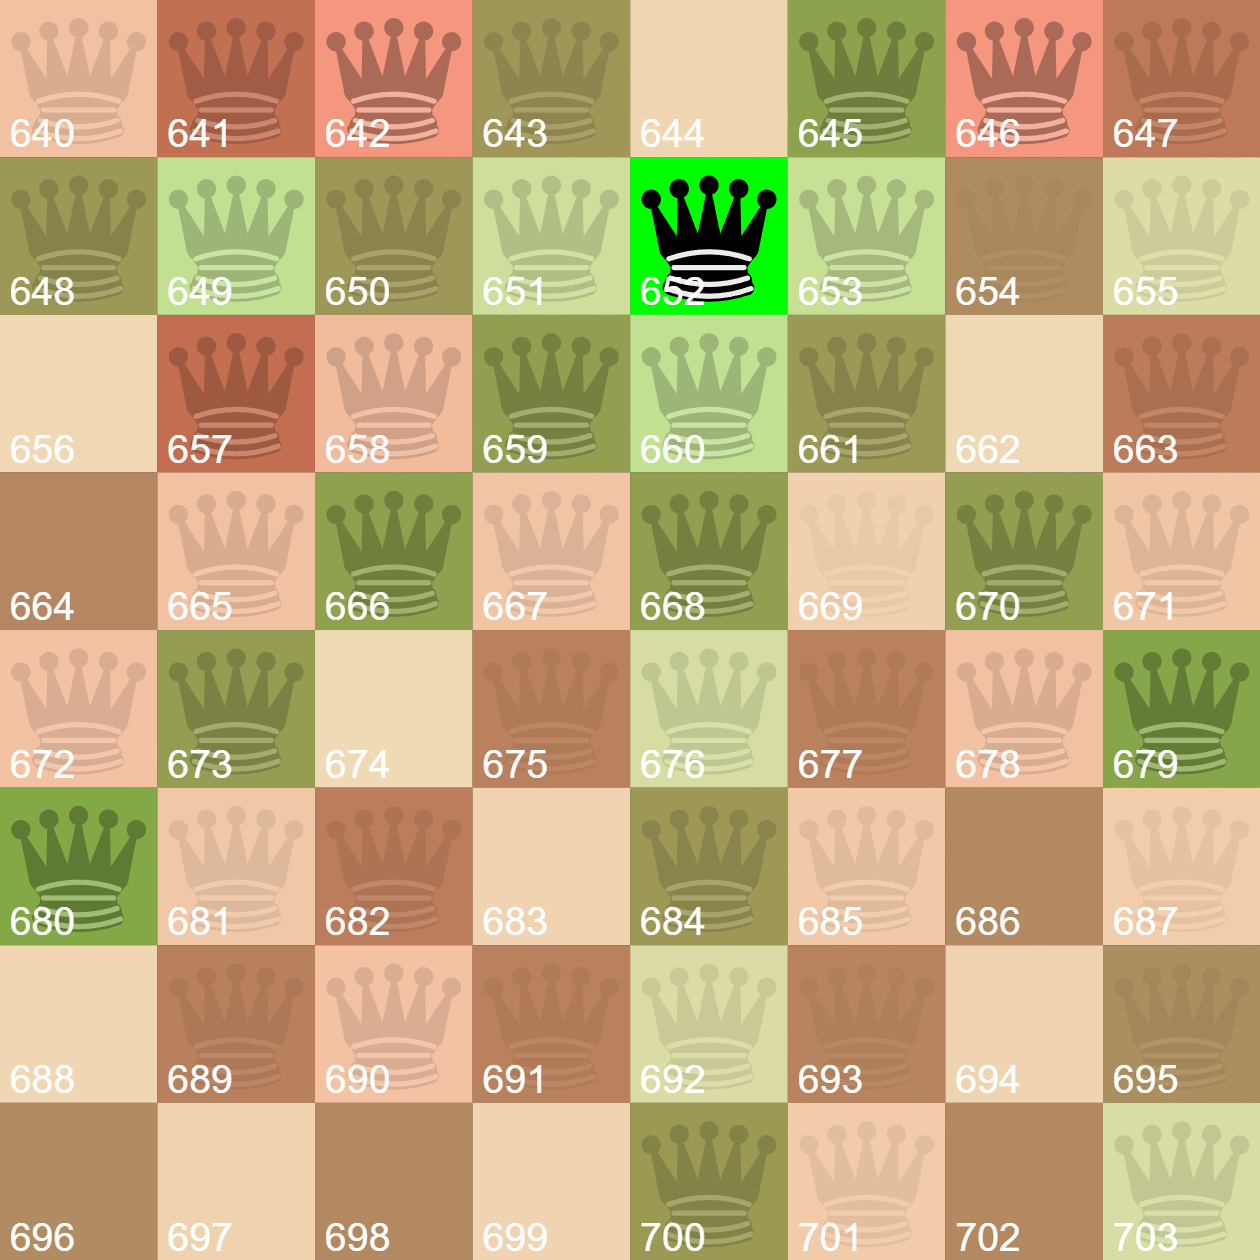
\includegraphics[width=4.65cm]{../assets/results/piece_weights/black_queen_weights.png} }}
\qquad
\subfloat[\centering $\black$ Black]{{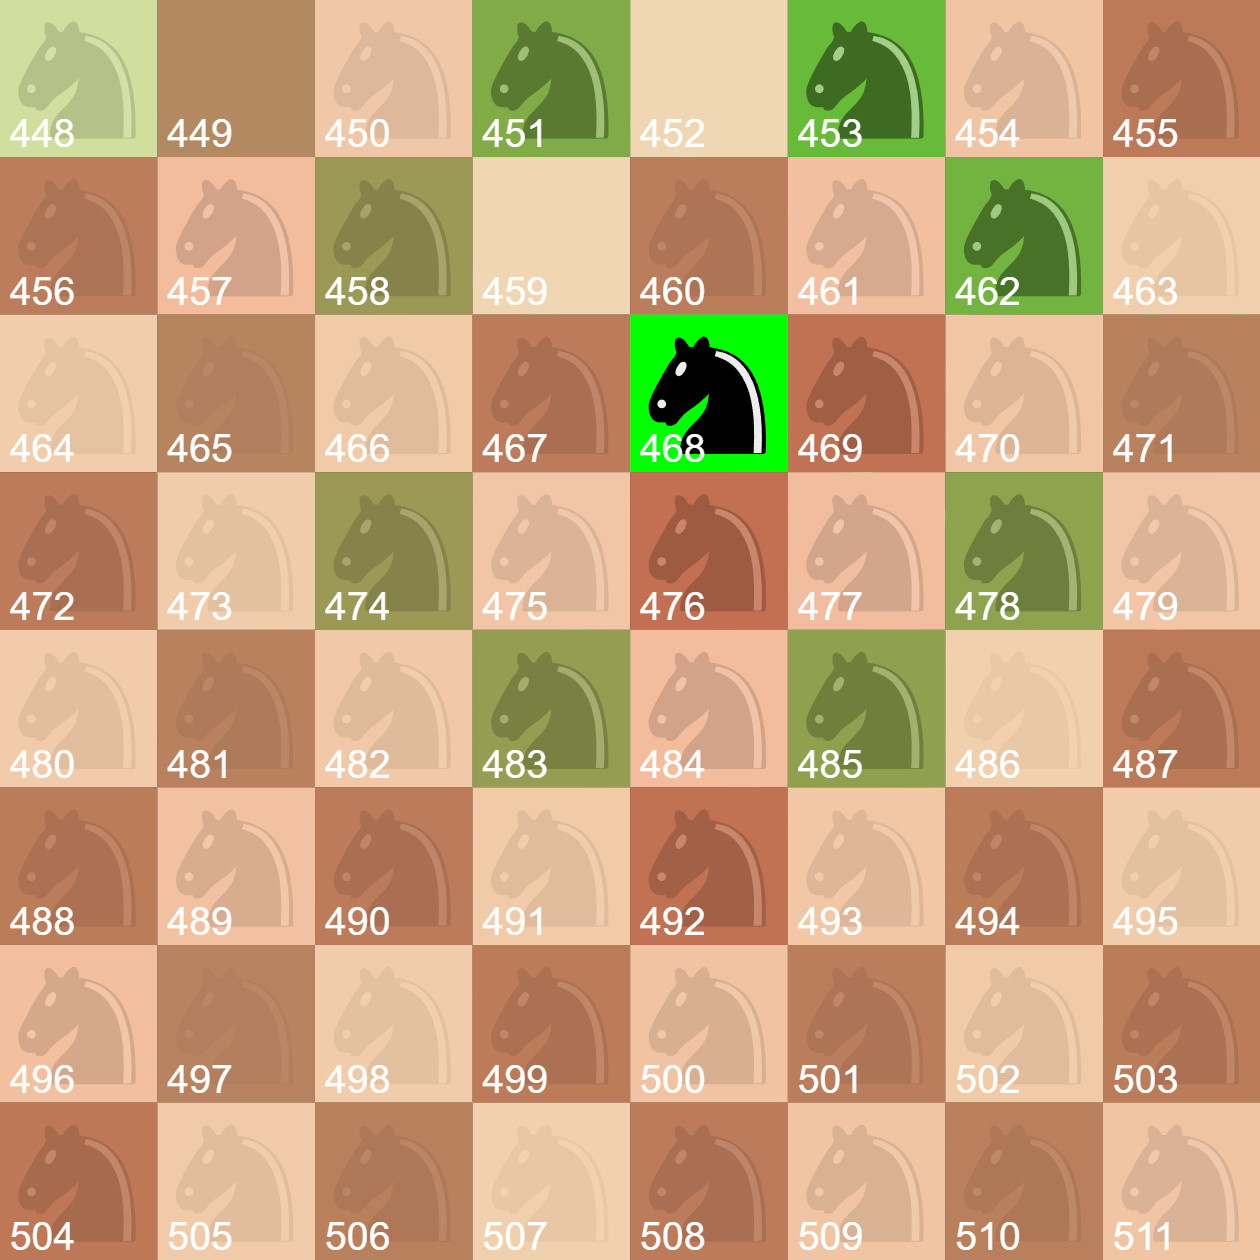
\includegraphics[width=4.65cm]{../assets/results/piece_weights/black_knight_weights.png} }} \\

\caption{Weights of different neurons in the L1 layer, which are connected to features in \featureset{Piece} with different roles. The intensity represents the weight value, and the color represents the sign. The number is the feature index, specifically \featureset{VH} instead of \featureset{HV} (both are \featureset{Piece}), because it was prior to the first experiment. Refer to section \ref{sec:axis_encoding}.}
\end{figure}
